\chapter{Einleitung}

Die Sprache des Menschen ist die natürlichste Art und Weise um miteinander zu kommunizieren \cite{spectrogram}. Durch die technische Entwicklung in den letzten Jahren kommen immer mehr Interaktionen zwischen Mensch und Maschine durch die Sprache zustande. Die Bezeichnung dafür sind die sogenannten intelligent personal assistants (IPAs) \cite{badshah2019deep} wie zum Beispiel Amazon Alexa, Apple Siri und Google Assistant. Google Home, Amazon Echo und Apple HomePod sind Home-Assistant Systeme, die primär Sprachsignale als Interaktionsmöglichkeit besitzen. Diese IPAs sind sehr stark verbreitet und auf vielen Geräten verfügbar \cite{speech_in_hci}.


\section{Was ist speech emotions recognition (SER)}
SER ist ein Forschungsgebiet, welches sich mit der Analyse von Audiosignalen, durch das Extrahieren von typischen Merkmalen und anschließender Klassifikation der Emotionen, beschäftigt \cite{spectrogram}. In den letzten Jahren wurden in diesem Gebiet von Spracherkennung signifikante Fortschritte gemacht. Die Audiosignale enthalten nicht nur die gesprochenen Wörter, sondern vielmehr auch den emotionalen Zustand des Sprechers \cite{badshah2019deep,speech_in_hci}. Das Ziel hierbei ist es durch verschiedene Klassifikationsverfahren das menschliche Befinden, die Gefühle und die Emotionen aus den Audiosignalen zu extrahieren und somit den emotionalen Zustand des Sprechers vorherzusagen \cite{spectrogram}. SER kann zum Beispiel als diagnostisches Werkzeug für Therapeuten verwendet werden. Eine weitere Einsatzmöglichkeit bietet SER bei Notrufzentralen, um die Ernsthaftigkeit der Situation des Anrufenden maschinell durch die Stimme erkennen zu können \cite{badshah2019deep}. Bei SER-Systemen gibt es verschiedene Herausforderungen wie zum Beispiel  Robustheit bei Tonänderungen, unterschiedliche Sprechstile, Anzahl der Wörter und kulturell bedingte Ausdrucksweise der Emotionen beim Sprechen \cite{spectrogram}. Allgemein werden Emotionen bei SER in 2 Hauptkategorien unterteilt - bewusst und unbewusst ausgedrückte Emotionen \cite{elearning}. Bewusst ausgedrückte Emotionen sind offensichtlicher als unbewusst ausgedrückte Emotionen. Wenn jemand beim Sprechen mit der Stimme lauter wird, so ist dies ein Indikator dafür, dass der Sprecher wütend ist. Dies ist ein Beispiel für bewusst ausgedrückte Emotionen. Der Sprecher kann aber auch wütend sein ohne seine Stimme zu erheben, da müssen dann andere Indikatoren hergezogen werden wie zum Beispiel die Knappheit der Wörter \cite{elearning}. Somit ist das Hauptproblem von SER-Systemen die Erkennung von affektorientierte Unterscheidungsmerkmale der Sprachsignale und welche Kriterien zur Vorhersage für die Emotionen des Sprechers dienen \cite{badshah2019deep}.

\section{Spektrogramme}
Spektrogramme kommen in verschiedenen Sprachanalyse-Tools zum Einsatz wie zum Beispiel bei Sound Event Classification (SEC), Sprecher Erkennung, Spracherkennung und SER \cite{spectrogram}.
Bei SER-Systemen dienen Spektrogramme als Input in das Convolutional Neural Network (CNN) \cite{cnn}, welche aus den Sprachsignalen generiert werden. 
Ein Spektrogramm ist eine visuelle Darstellung der Audiosignale in Form von zweidimensionalen Graphen \cite{spectrogram}. Dieser Graph hat folgende geometrische Dimensionen: die horizontale Achse repräsentiert die Zeit t und die vertikale Achse bildet die zeitabhängige Frequenz des Audiosignals \cite{badshah2019deep}. Die Amplitude der Frequenz wird durch unterschiedliche Farben in der Darstellung gezeigt: niedrige Amplituden werden durch dunkelblaue Farben und hohe Amplituden durch hellere Farben bis hin zu Rot dargestellt (siehe Abbildung \ref{spektogram}) \cite{spectrogram}. Somit entsteht eine Wellenform über die Zeit, was die Audiosignale des Sprechers repräsentiert und wichtige Informationen enthält. 
\begin{figure}[ht]
	\centering
	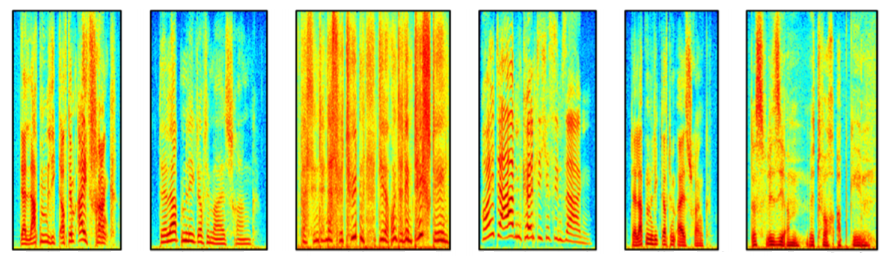
\includegraphics[width=1\textwidth]{images/spekto.PNG}
	\caption{\label{spektogram}Spektogramme für verschiedene Emotionen \cite{badshah2019deep}}
\end{figure}
\subsection{STFT und FFT}
STFT steht für short term Fourier transform und wird für elektronisch aufgezeichnete Tonaufnahmen verwendet, um aus den Signalen ein Spektrogramm zu generieren \cite{badshah2019deep}. Bei fast Fourier transform (FFT) handelt es sich um einen digitalen Prozess, welcher die Signale über ein sich gleitendes Fenster berechnet und damit ein Spektrogramm erstellt \cite{badshah2019deep}. Bei der Erstellung der Spektrogramme im Paper \cite{badshah2019deep} wurden Sprachaufnahmen von Emo-DB (Berlin Database of Emotional Speech) mit dem STFT-Algorithmus in Spektrogrammen umgewandelt, um später sie als Input für das Convolutional Neural Network zu verwenden.
%Bilder kann man natürlich auch in Arbeiten integrieren. Für Fotos und ähnliches %unterstützt PDF-\LaTeX{} direkt \verb|jpg| und \verb|png|, ansonsten empfiehlt es sich %Vektorgrafiken zu verwenden und diese als \verb|pdf| zu speichern. Sollte ein Bild %einmal zu viel weißen Raum um sich haben, so kann man mit dem Werkzeug \verb|pdfcrop| %das Bild automatisch ausschneiden

%\begin{figure}[ht]
%    \centering
%    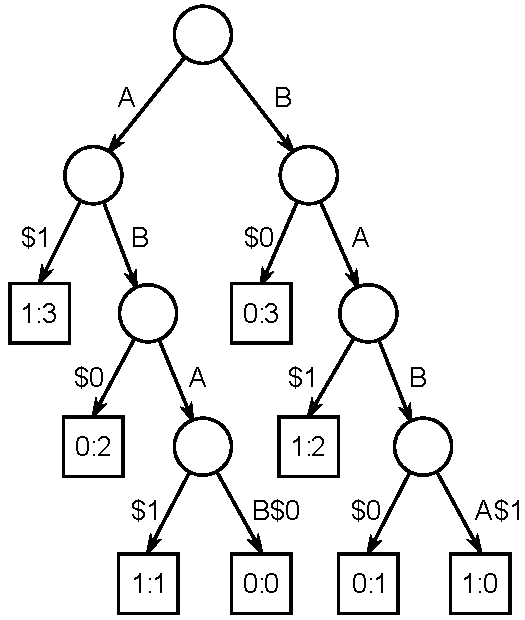
\includegraphics[width=.4\textwidth]{images/Suffix_tree_ABAB_BABA}
%    \caption{\label{anker}Bechreibung des Bilds}
%\end{figure}

%Mit Hilfe eines Labels kann man sich dann im Text auf diese Grafik (\ref{anker}) %beziehen. 

%\begin{figure}[ht]
%    \centering
%    \subfigure[Ein fettes u]{
%        
\includegraphics[width=0.2\linewidth]{images/a}
%        \label{subfigurebsp:a}
%    }
%    \hspace{1cm}
%    \subfigure[Ein dünneres u]{
%        
\includegraphics[width=0.2\linewidth]{images/b}
%        \label{subfigurebsp:b}
%    }
%    \caption{Die \emph{u}s aus der Wortmarke}
%\end{figure}

%Durch \verb|subfigure| lassen sich auch zwei kleine Bilder nebeneinander setzen. In %Abbildung \ref{subfigurebsp:a} ist ein fettes u auf der linken und in %\ref{subfigurebsp:b} ein dünneres auf der rechten Seite zu sehen.


%\subsection{Tabellen}

%Hier nur ein kurzes Beispiel, in jedem \LaTeX{} Buch finden sich gute Anleitungen zum %Erstellen von Tabellen.

%\begin{table}[h]
%    \centering
%    \begin{tabular}{|l|l|l|}
%        A & B & C \\
%        \hline
%        x & x & x \\
%        x & x & x
%    \end{tabular}
%\end{table}


%\subsection{Formeln}

%Mathematische Formeln lassen sich als Umgebung mit \verb|\begin{math}| und \verb|\end{math}| erzeugen, es gibt aber auch eine abgekürzte Schreibweise mit \verb|\( Formel \)| wobei die Formel dann im laufenden Text bleibt. Die kürzeste Form ist mit zwei \verb|$| um die Formel, z.B.~so Wasser ist H$_2$O.

%Mit der Schreibweise \verb|\[ Formel \]| wird die Formel mittig auf einer neuen Zeile gesetzt, z.B.

%\[y = x^2 \]

%Dies ist die Kurzform der Umgebung \verb|equation|, mit der die Gleichung auch nummeriert wird. 

%\begin{equation}
%    x_{1,2} = \frac{-b\pm\sqrt{b^2-4ac}}{2a}
%    \label{mitternachtsformel}
%\end{equation}

%Wenn wir z.B.~über die beliebte Mitternachtsformel (Gleichung \ref{mitternachtsformel}) schreiben wollen lässt sich diese also wie ein Bild referenzieren.



